\documentclass[a4paper,11pt]{article}
\usepackage[utf8]{inputenc}
\usepackage{amsmath}
\usepackage{amssymb}
\usepackage[hidelinks]{hyperref}
\usepackage{geometry}
\geometry{margin=1in}
\usepackage{enumitem}
\usepackage{xcolor}
\usepackage{graphicx}
\usepackage{float}

\title{CSCib Lab Checklist}
\author{}
\date{}

\begin{document}
\maketitle

\section*{Checklist transversal: preparar a pasta de trabalho}

Aplica-se a todas as sessões de laboratório (L2, L3, e seguintes), antes de começar
qualquer tarefa no MATLAB.

\begin{enumerate}[label=$\square$, leftmargin=1.5em]
  \item Abrir o MATLAB, confirmando que é a versão correta, \textbf{R2015a} (versão 8).
  Se houver mais do que uma versão instalada no PC do laboratório, escolher sempre
  esta, para garantir compatibilidade com o resto do trabalho.

  \item Criar, no Desktop do PC do laboratório, uma pasta com nome identificável,
  incluindo o número do grupo e a sessão. Exemplo: \texttt{Desktop\textbackslash
  CSCib\_GrupoXX\_L2}.

  \item Confirmar que essa pasta tem permissões de escrita, criando um ficheiro de
  teste qualquer dentro dela e apagando a seguir. O guia pede explicitamente que se
  use "a working folder with write permissions".

  \item Definir essa pasta como \emph{Current Folder} no MATLAB. Usar o campo
  "Current Folder" da barra de ferramentas, ou o comando:
  \begin{verbatim}
cd('Desktop\CSCib_GrupoXX_L2')
  \end{verbatim}
  Não confundir com "Set Path": este serve para indicar ao MATLAB onde procurar
  funções, não onde gravar ficheiros.

  \item Confirmar o caminho correto antes de gravar qualquer coisa:
  \begin{verbatim}
pwd
  \end{verbatim}

  \item Gravar sempre os dados com o comando direto. Exemplo:
  \begin{verbatim}
save('input.mat', 'input')
  \end{verbatim}

  \item No final da sessão, copiar a pasta completa para a pen, e apagar essa pasta
  do PC do laboratório (limpeza obrigatória, pedida pelo guia).
\end{enumerate}

\section*{Checklist L2: enviar comandos ao motor (Secção 3.3 do guia)}

\textcolor{red}{\textbf{Avisos de segurança, válidos a partir daqui:}} manter distância
de segurança da barra flexível; ter sempre um dedo perto do interruptor do
amplificador de potência para poder parar o motor; nunca deixar a barra rodar sobre
si própria.

\begin{enumerate}[label=$\square$, leftmargin=1.5em]
  \item Copiar da pen para a pasta de trabalho (já criada na checklist transversal)
  o ficheiro \texttt{.slx} feito em casa, com o modelo dos passos 1 a 7 (Signal
  Generator ligado a um Scope, com o sinal a gravar em \texttt{input}). Abrir esse
  ficheiro no MATLAB. Não é preciso recomeçar o modelo do zero, só continuar a
  construir sobre ele.

  \item Inserir um bloco D/A: \texttt{Simulink Desktop Real-Time} $\to$
  \texttt{Analog Output}. Ligar o Signal Generator a este bloco.

  \item Identificar a placa de aquisição de dados instalada: olhar para a parte de
  trás do computador da bancada e localizar o conector da placa. Se a ligação for
  prateada, a placa é a \textbf{NI PCI-6221}. Se a ligação for azul, a placa é a
  \textbf{NI MIO16E4}. Anotar qual é.

  \item Configurar o bloco D/A: selecionar a placa identificada no passo anterior,
  sample time \texttt{0.001}, output channel \texttt{1}, voltage range de $-10$ a
  $10$ V, data type \texttt{volts}. \textcolor{red}{\textbf{Valor inicial e valor
  final devem ser exatamente 0.}} Se o valor final não for zero, o motor fica a
  rodar sem parar no fim da experiência e pode danificar o equipamento.

  \item Configurar a simulação para tempo real (\texttt{Ctrl+E}):
  \begin{itemize}
    \item Solver: Type = \texttt{Fixed-step}.
    \item Code Generation: System Target File = \texttt{rtwin.tlc}.
    \item Hardware Implementation: Device vendor = \texttt{Intel}, Device type =
    \texttt{X86/Pentium}.
  \end{itemize}

  \begin{figure}[H]
    \centering
    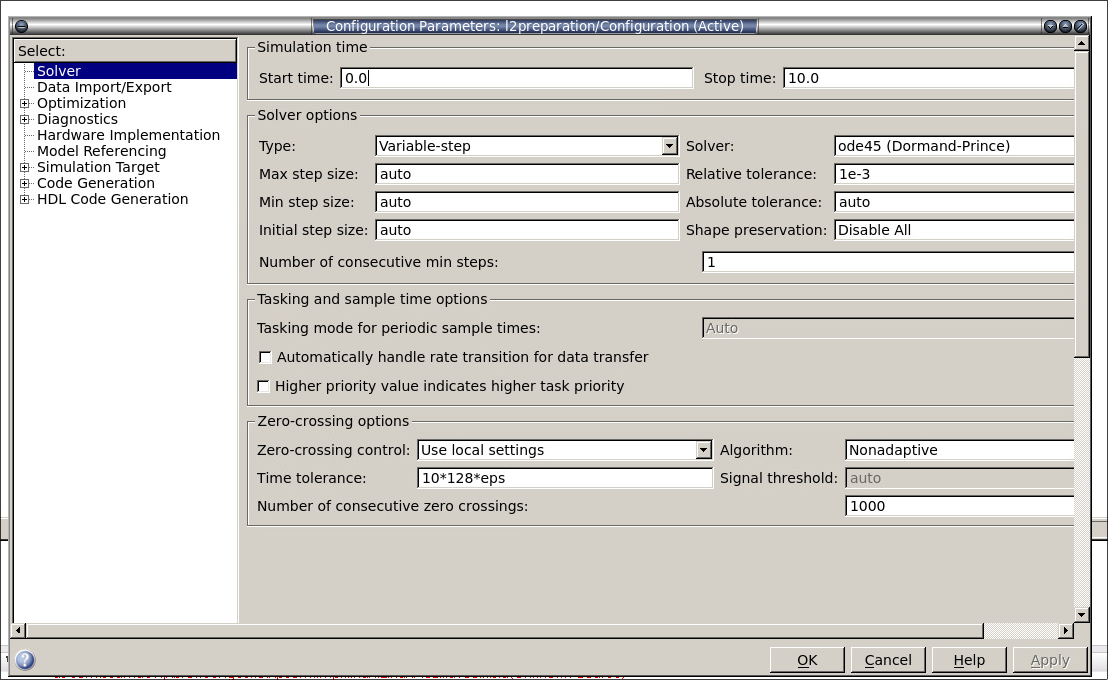
\includegraphics[width=0.85\textwidth]{Figs/l2_solver_config.png}
    \caption{Painel \emph{Solver} em \emph{Configuration Parameters}. Nesta captura
    o \texttt{Type} ainda está em \texttt{Variable-step} (valor por omissão);
    mudar para \texttt{Fixed-step}, conforme pedido acima.}
  \end{figure}

  \item Configurar o modo \emph{External}: menu \emph{Code}, depois \emph{External
  Mode Control Panel}, depois \emph{Signal \& Triggering}. Duration =
  \texttt{10001} amostras (10 segundos a 1000 amostras por segundo, mais a amostra
  inicial). Confirmar, na barra de comandos do Simulink, que o modo selecionado é
  \texttt{External}.

  \begin{figure}[H]
    \centering
    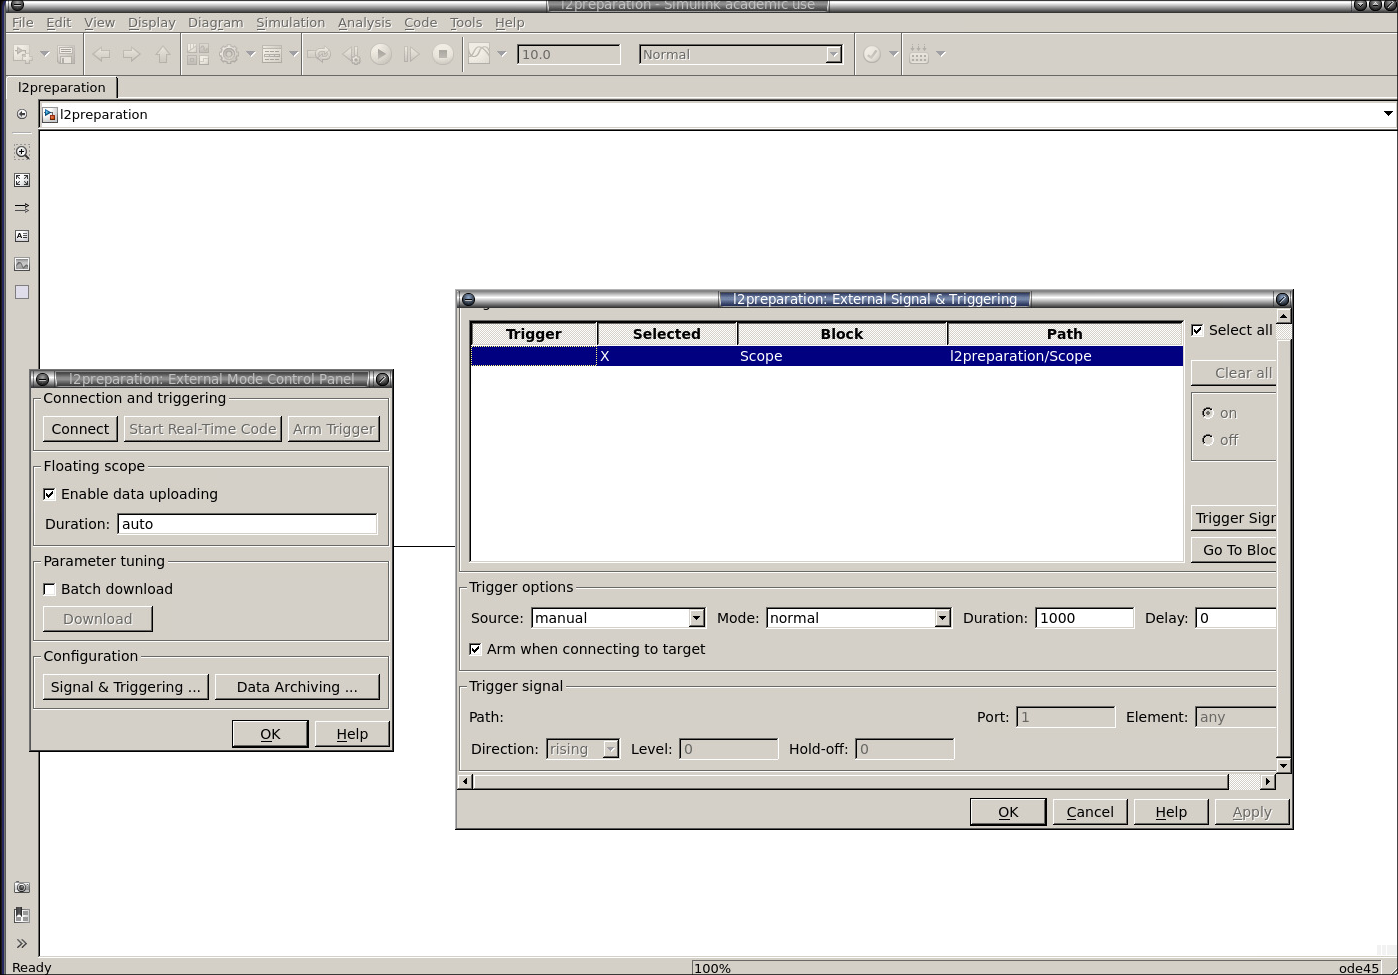
\includegraphics[width=0.95\textwidth]{Figs/l2_external_mode.png}
    \caption{\emph{External Mode Control Panel} (canto inferior esquerdo, acedido
    pelo menu \emph{Code}) e \emph{External Signal \& Triggering} (à direita, botão
    \emph{Signal \& Triggering...}). Nesta captura, \texttt{Duration} está em
    \texttt{1000}; mudar para \texttt{10001}, conforme pedido acima.}
  \end{figure}

  \item Gravar o projeto na pasta de trabalho.

  \item Pedir à equipa do laboratório para confirmar que está tudo corretamente
  configurado, antes de correr qualquer coisa.

  \item Correr a experiência (botão $\blacktriangleright$). Observar o
  comportamento do motor: dentro de cada meio período da onda quadrada, a tensão
  aplicada é constante, e nesse intervalo a posição angular não estabiliza,
  sobe ou desce continuamente até o sinal inverter (o mesmo efeito já discutido
  nas alíneas (a) e (b) da Q1, e ilustrado na Figura 11 do guia). Parar com o
  botão $\blacksquare$ quando necessário. Registar o que foi observado.

  \item No final, seguir novamente os dois últimos pontos da checklist transversal:
  copiar a pasta de trabalho para a pen, e apagar do PC do laboratório.
\end{enumerate}

\section*{Checklist L3: leitura de sensores e calibração (Secções 3.4 e 3.5 do guia)}

Avisos de segurança: os mesmos indicados na secção do L2, válidos também aqui.

\begin{enumerate}[label=$\square$, leftmargin=1.5em]
  \item Copiar da pen para a pasta de trabalho desta sessão o ficheiro \texttt{.slx}
  do L2 (já com o Signal Generator e o bloco D/A configurados). Abrir esse ficheiro
  e continuar a construir sobre ele, sem recomeçar do zero.

  \item Inserir um bloco A/D para o potenciómetro: \texttt{Simulink Desktop
  Real-Time} $\to$ \texttt{Analog Input}. Configurar: selecionar a placa de
  aquisição identificada no L2, sample time \texttt{0.001}, input channel
  \texttt{1} (potenciómetro), voltage range de $-10$ a $10$ V, data type
  \texttt{volts}.

  \item Inserir um bloco Scope para mostrar o sinal do sensor, configurado da mesma
  forma que o Scope do L2 (sample time \texttt{0.001}, "Save data to workspace"
  ativado). Dar à variável o nome \texttt{tensao\_pot}.

  \item Pedir confirmação à equipa do laboratório antes de correr. Correr a
  experiência, observar o gráfico da tensão do potenciómetro ao longo do tempo, e
  confirmar que a variável \texttt{tensao\_pot} está disponível no workspace do
  MATLAB. Gravar:
  \begin{verbatim}
save('tensao_pot.mat', 'tensao_pot')
  \end{verbatim}

  \item \textbf{Calibração de $K_p$ (sem a barra montada no motor):} desmontar a
  barra do veio do motor antes de continuar.

  \item Aplicar um degrau de $1$ V ao motor (o mesmo bloco D/A, agora com um valor
  constante em vez do Signal Generator) e deixar o motor rodar livremente durante
  alguns segundos, registando \texttt{tensao\_pot} continuamente.

  \item No MATLAB, processar os dados para obter $K_p$:
  \begin{enumerate}[label=(\alph*)]
    \item Detetar os instantes de reset do sinal (onde a tensão salta de um
    extremo para o outro), com \texttt{diff} e um limiar adequado.
    \item Descartar o primeiro ciclo (motor ainda em transitório de arranque).
    \item Ajustar uma reta aos pontos (instante do reset, número de rotações
    acumuladas $\times$ $360^\circ$) para estimar a velocidade angular $\omega$, usando
    todos os resets detetados.
    \item Calcular, para cada amostra, o ângulo de referência local $\theta_{\text{ref}}(t)
    = \omega \cdot (t - t_k)$, onde $t_k$ é o reset imediatamente anterior à
    amostra.
    \item Ajustar por mínimos quadrados $\theta_{\text{ref}} = K_p \cdot \theta_e +
    \text{offset}$, juntando os dados de todos os ciclos (\texttt{polyfit} ou o
    operador \texttt{\textbackslash}).
  \end{enumerate}

  \item \textbf{Calibração de $K_e$ (barra na bancada de calibração, não no
  motor):} montar a barra na bancada com o pente de calibração, e ligar o cabo ao
  extensómetro (não ao potenciómetro).

  \item Continuar no mesmo modelo base (não criar um ficheiro novo): adicionar um
  bloco \texttt{Analog Input} para o extensómetro, juntando-se ao Signal Generator,
  ao D/A e ao Analog Input do potenciómetro já existentes, exatamente como na
  Figura 10 do guia. O Signal Generator e o D/A ficam sem função relevante nesta
  calibração (a barra está desligada do motor), mas não é preciso removê-los.

  \begin{figure}[H]
    \centering
    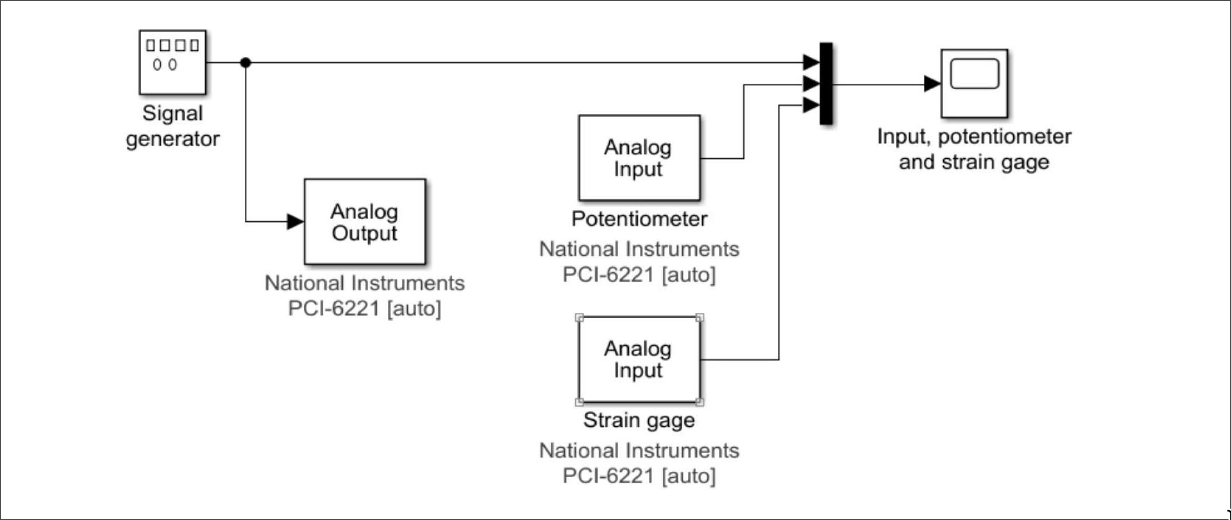
\includegraphics[width=0.95\textwidth]{Figs/l3_full_diagram.png}
    \caption{Diagrama completo (Figura 10 do guia): Signal Generator ligado ao D/A
    (\emph{Analog Output}), e dois blocos \emph{Analog Input}, um para o
    potenciómetro e outro para o extensómetro, ambos juntados num Mux antes do
    Scope final.}
  \end{figure}

  \item Configurar o novo bloco A/D, com os mesmos parâmetros do bloco do
  potenciómetro (passo 15 do guia): sample time \texttt{0.001}, voltage range de
  $-10$ a $10$ V, data type \texttt{volts}. \textbf{Atenção:} o guia não indica por
  escrito o número do canal do extensómetro (só o do potenciómetro, canal
  \texttt{1}). Confirmar na bancada qual o canal correto (etiqueta do conector, ou
  perguntar à equipa do laboratório) antes de escolher no bloco.

  \item Inserir um bloco Scope (ou display) ligado a este novo A/D, para ler a
  tensão do extensómetro.

  \item Para cada ranhura do pente, defletir a barra até essa ranhura e registar a
  tensão elétrica correspondente. Calcular o ângulo de deflexão de cada ranhura por
  $\alpha_{\text{[graus]}} = \frac{180}{\pi} \cdot \frac{D}{L}$, com $D$ a distância
  de deflexão da ranhura e $L$ o comprimento da barra.

  As ranhuras do pente estão espaçadas em intervalos de $1/4$ polegada
  ($0.635$ cm $= 6.35$ mm), pelo que a distância de deflexão da ranhura número $n$
  (contada a partir da posição de repouso) é:
  $$D_n = n \times 6.35 \text{ mm}$$

  Usar a tabela seguinte (preenchida à mão, rapidamente, junto à bancada):

  \begin{table}[H]
    \centering
    \renewcommand{\arraystretch}{2.2}
    \begin{tabular}{|c|c|c|c|}
      \hline
      \textbf{Ranhura} & \textbf{$D$ (mm)} & \textbf{$\alpha$ (graus)} &
      \textbf{Tensão medida (V)} \\
      \hline
       & & & \\
      \hline
       & & & \\
      \hline
       & & & \\
      \hline
       & & & \\
      \hline
       & & & \\
      \hline
       & & & \\
      \hline
       & & & \\
      \hline
       & & & \\
      \hline
       & & & \\
      \hline
       & & & \\
      \hline
    \end{tabular}
    \caption{Tabela de calibração de $K_e$: deflexão do pente contra tensão
    medida.}
  \end{table}

  \item Com os pares $(\alpha, \text{tensão})$ da tabela, ajustar por mínimos
  quadrados $\alpha = K_e \cdot \alpha_e + \text{offset}$ no MATLAB, e gravar os
  dados brutos usados no ajuste.

  \item No final, seguir novamente os dois últimos pontos da checklist
  transversal: copiar a pasta de trabalho para a pen, e apagar do PC do
  laboratório.
\end{enumerate}

\end{document}
